%%%%%%%%%%%%%%%%%%%%%%%%%%%%%%%%%%%%%%%%%%%%%%%%%%%%%%%%%%%%%%%%%%%%%%%%%%%%%%%
% PHD PROJECT IN QUANTUM DYNAMICS - REVISED VERSION
% Quantum Engineering of Symbiotic Agrivoltaic Systems
% Written by S. G. Nana Engo for Théodore Fredy Goumai
% Date: 05 October 2025
%%%%%%%%%%%%%%%%%%%%%%%%%%%%%%%%%%%%%%%%%%%%%%%%%%%%%%%%%%%%%%%%%%%%%%%%%%%%%%%

\documentclass[12pt, a4paper]{article}

% --- ESSENTIAL PACKAGES ---
\usepackage[utf8]{inputenc}
\usepackage[T1]{fontenc}
\usepackage[english]{babel}
\usepackage[margin=2.cm]{geometry}

% --- SCIENTIFIC AND FORMATTING PACKAGES ---
\usepackage{amsmath, amssymb}
\usepackage{graphicx, booktabs, tabularx, xcolor, longtable, multirow}
% caption handling for tables and figures
\usepackage[bf,textfont={footnotesize,it}]{caption}
% appendices management
\usepackage[toc,page,title,titletoc,header]{appendix}

% --- SPECIALIZED PACKAGES ---
\usepackage{physics} % bra-ket, abs, norm, etc.
\usepackage{hyperref} % hyperlinks
\usepackage{cleveref} % smart references (\Cref)

\usepackage[
  locale=US,
  detect-all=true,
  group-minimum-digits=4,
  separate-uncertainty=true,
  multi-part-units=single,
  range-phrase=--,
  range-units=single,
  number-unit-product=\,]{siunitx}

% Diagrams
\usepackage{tikz}
\usetikzlibrary{shapes.geometric, arrows, positioning, calc}

% --- GLOBAL CONFIGURATIONS ---

% Hyperlink configuration
\hypersetup{
    colorlinks=true,             % colored links rather than boxed
    linkcolor=blue!50!black,     % internal links (sections, figures)
    citecolor=green!50!black,    % citation color
    urlcolor=blue!80!black,      % URL color
    pdftitle={PhD Project - Quantum Engineering of Symbiotic Agrivoltaic Systems},
    pdfauthor={Théodore Fredy Goumai}
}

% Custom units for siunitx
\DeclareSIUnit{\year}{yr}
\DeclareSIUnit{\dollar}{\$}
\DeclareSIUnit{\euro}{€}

%%%%%%%%%%%%%%%%%%%%%%%%%%%%%%%%%%%%%%%%%%%%%%%%%%%%%%%%%%%%%%%%%%%%%%%%%%%%%%%
% BEGIN DOCUMENT
%%%%%%%%%%%%%%%%%%%%%%%%%%%%%%%%%%%%%%%%%%%%%%%%%%%%%%%%%%%%%%%%%%%%%%%%%%%%%%%
\begin{document}

\title{\huge Quantum engineering of symbiotic agrivoltaic systems:\\ From excitonic coherence to the eco-design of photonic materials}
\author{
    Théodore Fredy Goumai (Doctoral Candidate) \\
    \\
    \textit{Under the supervision of} \\
    J.-P. Tchapet Njafa, PhD \\
    S. G. Nana Engo, Professor
}
\date{October 2025}

\maketitle
\thispagestyle{empty}
\newpage

\begin{abstract}
This doctoral project introduces a novel framework for the design of symbiotic quantum agrivoltaic systems, combining advanced non-Markovian quantum dynamics, photonic materials engineering, and ethical artificial intelligence. We develop a unified approach that models cropping under panels as an open quantum system subject to a filtered photonic bath, formalizing for the first time the coherent coupling between excitonic energy transfer (\texttt{EET}) and plant photosynthesis. The methodological architecture integrates \texttt{Process Tensor-HOPS} and \texttt{Stochastically Bundled Dissipators} to enable realistic mesoscale quantum simulation, coupled to a generative AI pipeline for the design of non-toxic and biodegradable organic photovoltaic (\texttt{OPV}) materials. The project establishes an open-source quantum software ecosystem, \texttt{AgroQuantPV Suite}, and experimentally demonstrates the simultaneous optimization of energy output (\texttt{PCE} > \SI{20}{\percent}) and agricultural performance (\texttt{ETR\_{rel}} > \SI{90}{\percent}) via adaptive spectral control. The impact is quantified across eleven Sustainable Development Goals, with a valorization pathway through the \texttt{AgroQuantum Technologies} spin-off targeting a levelized cost of energy (\texttt{LCOE}) of \SI{0.04}{\dollar\per\kilo\watt\hour}.
\end{abstract}
\newpage

\tableofcontents
\newpage
\setcounter{page}{1}

\section{Background, state of the art, and project positioning}

The global energy transition requires photovoltaic conversion technologies that are not only efficient but also sustainable and integrated with existing ecosystems. At the core of these technologies, charge-transport and charge-separation processes are governed by complex quantum dynamics strongly coupled to a thermo-vibrational environment \cite{ye2012, mohs2008}. This project is positioned at the intersection of quantum physics, materials science, and agronomy, within the emerging field of \textbf{Quantum Energy Science} \cite{Metzler2023}. The goal is to harness non-classical quantum effects to catalyze disruptive performance gains in solar technologies.

The 2024–2025 state of the art is marked by significant advances that redefine the boundaries of simulation and materials design:
\begin{itemize}
  \item \textbf{Process Tensor} methods are emerging as a formally exact solution for modeling non-Markovian quantum memory, surpassing the limitations of traditional hierarchical approaches \cite{keeling2025}.

  \item \textbf{Stochastically Bundled Dissipators} offer a promising route to drastically reduce the cost of simulating Lindblad dynamics for very large systems \cite{Adhikari2025}.

  \item \textbf{3D multi-layer architectures} for solar collection enable unprecedented spectral optimization, opening the way to high value-added applications \cite{shi2025a}.

  \item \textbf{Additive manufacturing (3D printing)} of OPV materials has reached a maturity that enables large-scale, local, and lower-cost production \cite{ju2025}.

  \item \textbf{Quantum software ecosystems} are beginning to integrate the entire value chain, from fundamental computation to industrial applications, fostering a hardware–software co-design approach \cite{basermann2024}.
\end{itemize}

In response to these advances, this project proposes to take a further step by integrating them within a holistic vision: \textbf{next-generation quantum agrivoltaics}. The aim is to mobilize these cutting-edge tools not merely to improve a single component, but to design a symbiotic system in which clean energy production and food security mutually reinforce each other. The objective is to create transparent, spectrally selective, economically viable, and socially responsible agrivoltaic systems, as illustrated in \Cref{fig_agrivoltaic_3d}.

\begin{figure}[htb]
    \centering
    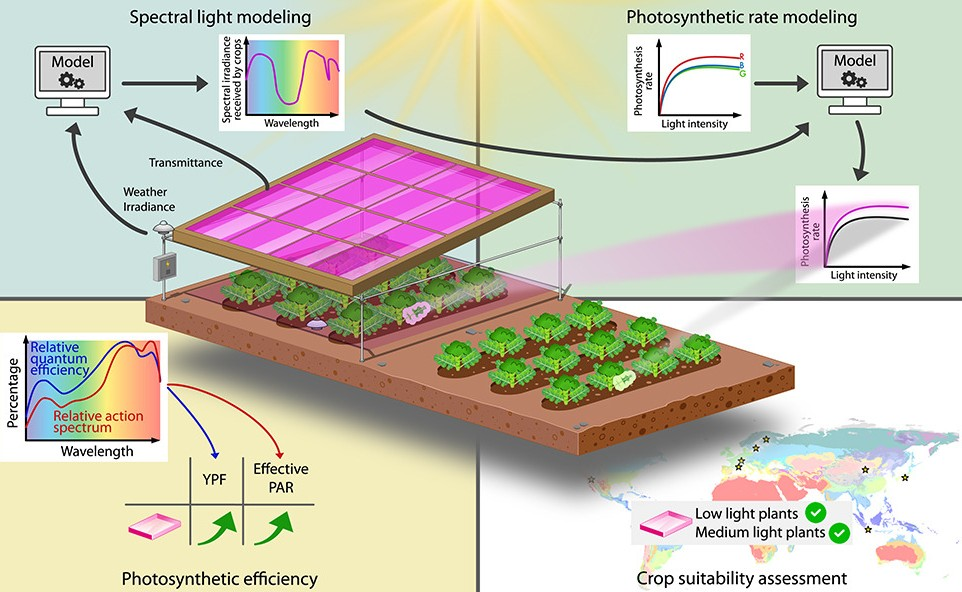
\includegraphics[width=0.8\textwidth]{agri-photovoltaic.jpg}
    \caption{3D vision of quantum agrivoltaics: transparent multi-layer panels with integrated quantum sensors.}
    \label{fig_agrivoltaic_3d}
\end{figure}

\section{Research problem}

The central challenge is to develop an integrated technology platform that leverages advances in non-Markovian quantum dynamics, artificial intelligence, and additive manufacturing to design next-generation agrivoltaic systems, addressing the following questions:
\begin{enumerate}
  \item How can \textit{Process Tensor Approaches} model quantum memory in complex photosynthetic and OPV systems with accuracy and efficiency superior to hierarchical methods?

  \item How can near real-time simulation of plot-scale systems (N \num{>1000} chromophores) be achieved via \textit{Stochastically Bundled Dissipators} while preserving non-Markovian effects?

  \item How can a 3D solar-harvesting architecture be optimized to simultaneously maximize energy production and agricultural productivity through adaptive spectral filtering?

  \item How can a quantum software ecosystem, the \textit{AgroQuantPV Suite}, be designed and deployed to facilitate industrial adoption and international collaboration?

  \item How can a technology transfer roadmap be established through a robust business plan and ethical governance?
\end{enumerate}

\section{Contribution to the Sustainable Development Goals (SDGs)}

This project is designed to generate measurable impact across eleven SDGs, with quantified metrics and contributions aligned with the official United Nations targets.

\subsection{SDG 7: Affordable and Clean Energy}
\begin{itemize}
    \item \textbf{Target 7.2.} Substantially increase the share of renewable energy in the global energy mix, aiming for an LCOE below \SI{0.04}{\dollar\per\kilo\watt\hour}.

    \item \textbf{Target 7.a.} Strengthen international cooperation to facilitate access to research and technology in clean energy via the open-source \textit{AgroQuantPV Suite} ecosystem.

    \item \textbf{Target 7.3.} Contribute to doubling the global rate of improvement in energy efficiency through a 3D architecture that increases collector area by more than \SI{60}{\percent}.
\end{itemize}

\subsection{SDG 2: Zero Hunger}
\begin{itemize}
    \item \textbf{Target 2.3.} Double agricultural productivity by maintaining \SI{90}{\percent} of the Electron Transport Rate (ETR) under the panels.

    \item \textbf{Target 2.4.} Ensure sustainable food production systems and implement resilient agricultural practices through 3D canopy monitoring with quantum sensors.
\end{itemize}

\subsection{SDG 3: Good Health and Well-Being}
\begin{itemize}
    \item \textbf{Target 3.9.} Substantially reduce the number of deaths and illnesses from hazardous chemicals and pollution by developing biodegradable OPV materials and an additive manufacturing process free of toxic solvents.
\end{itemize}

\subsection{SDG 6: Clean Water and Sanitation}
\begin{itemize}
    \item \textbf{Target 6.4.} Substantially increase water-use efficiency by reducing evaporation by \SI{25}{\percent}.

    \item \textbf{Target 6.6.} Protect and restore water-related ecosystems by establishing blockchain traceability for circular-material flows to avoid contamination.
\end{itemize}

\subsection{SDG 8: Decent Work and Economic Growth}
\begin{itemize}
    \item \textbf{Target 8.2.} Achieve higher levels of economic productivity through technological modernization and innovation by creating the \textit{AgroQuantum Technologies} spin-off (\num{20}+ direct jobs).

    \item \textbf{Target 8.5.} Achieve full and productive employment and decent work for all women and men, with a target of \SI{40}{\percent} women among the \num{50}+ trained individuals.
\end{itemize}

\subsection{SDG 9: Industry, Innovation and Infrastructure}
\begin{itemize}
    \item \textbf{Target 9.4.} Upgrade infrastructure and retrofit industries to make them sustainable via the quantum software ecosystem for industrial innovation.

    \item \textbf{Target 9.5.} Enhance scientific research and upgrade the technological capabilities of industrial sectors by fostering innovation through a global collaborative platform.
\end{itemize}

\subsection{SDG 12: Responsible Consumption and Production}
\begin{itemize}
    \item \textbf{Target 12.2.} Achieve the sustainable management and efficient use of natural resources through a circular economy for OPV materials.

    \item \textbf{Target 12.5.} Substantially reduce waste generation through prevention, reduction, recycling, and reuse via design-for-disassembly.
\end{itemize}

\subsection{SDG 13: Climate Action}
\begin{itemize}
    \item \textbf{Target 13.2.} Integrate climate change measures into policies, strategies, and planning through a \SI{60}{\percent} reduction in carbon footprint thanks to local additive manufacturing.
\end{itemize}

\subsection{SDG 15: Life on Land}
\begin{itemize}
    \item \textbf{Target 15.1.} Ensure the conservation, restoration, and sustainable use of terrestrial ecosystems by preserving \SI{100}{\percent} of agricultural land use.

    \item \textbf{Target 15.9.} Integrate ecosystem and biodiversity values into national and local planning by creating industry–agriculture symbiosis.
\end{itemize}

\subsection{SDG 16: Peace, Justice and Strong Institutions}
\begin{itemize}
    \item \textbf{Target 16.6.} Develop effective, accountable, and transparent institutions using blockchain for project governance.

    \item \textbf{Target 16.7.} Ensure responsive, inclusive, participatory, and representative decision-making by embedding AI ethics and environmental justice principles.
\end{itemize}

\subsection{SDG 17: Partnerships for the Goals}
\begin{itemize}
    \item \textbf{Target 17.6.} Enhance North–South and South–South cooperation in science, technology, and innovation via the \textit{AgroQuantPV Suite} ecosystem.

    \item \textbf{Target 17.9.} Strengthen international support for effective and targeted capacity-building through the creation of a global quantum-skills network.
\end{itemize}


\section{Thesis objectives: A holistic approach}

The project adopts a systemic view of sustainable technology development. Objectives are structured into three complementary axes, integrating technical refinements to ensure robustness and impact of the results.

\subsection{Axis 1: Innovations in quantum dynamics and modeling of symbiotic coupling}

This axis aims to develop a theoretical and computational framework capable of modeling, with unprecedented accuracy, the quantum dynamics of the coupling between excitonic energy (EET) in OPV materials and plant photosynthesis.

\subsubsection{Characterizing vibronic non-classicality as a driver of efficiency}
\begin{itemize}
    \item \textbf{Diagnosing non-classicality.} Quantify the non-classical nature of collective vibrational modes by incorporating advanced quantum diagnostics into the simulations, such as computing the \textbf{Mandel Q parameter} and the \textbf{Wigner quasi-probability distribution}.

    \item \textbf{Correlation with symbiotic performance.} Establish a direct correlation between the presence of vibronic non-classicality and the overall symbiotic efficiency (SPCE), to test the hypothesis that such quantum fluctuations are a key mechanism for energy optimization.
\end{itemize}

\subsubsection{High-fidelity simulation of structured thermal baths}
\begin{itemize}
    \item \textbf{Handling ultra-fast bath modes.} Implement and validate \textbf{Low-Temperature Correction (LTC)} techniques within the \texttt{HOPS} methodology. This approach will effectively treat Matsubara modes—crucial for spectroscopic benchmarks at \SI{77}{\kelvin}—while reducing computational cost without sacrificing accuracy.

    \item \textbf{Coupling beyond the point-dipole approximation.} Go beyond the ideal-dipole approximation (IDA) by systematically using the \textbf{Transition Density Cube (TDC)} method for intermolecular coupling ($J_{mn}$), ensuring accurate short-range interaction descriptions (\SI{<30}{\angstrom}) in OPV aggregates.
\end{itemize}

\subsubsection{Scalability to multi-excitation systems}
\begin{itemize}
\item Validate the Stochastically Bundled Dissipators (SBD) approach in the non-Markovian regime and exploit \texttt{MesoHOPS} scaling to address the challenge of double-excitation and charge-transfer states.
\end{itemize}

\subsection{Axis 2: 3D architecture and quantum sensors}

\subsubsection{Optimizing productive vibronic coherences}
\begin{itemize}
    \item \textbf{Spectral filtering for symbiosis.} Model the total transmittance $T_{\text{total}}(\omega) = \prod_{i=1}^N T_i(\omega, z_i)$ to identify quasi-resonances between excitonic transitions and functional vibrational modes, thereby maximizing vibration-assisted energy transfer.

    \item \textbf{Predictive canopy modeling.} Couple spectral-transmittance simulation to agronomic models (e.g., DSSAT) to predict the vertical ETR profile and optimize the energy–biomass trade-off.
\end{itemize}

\subsubsection{Probing system–environment quantum correlations}
\begin{itemize}
    \item \textbf{NV-center sensors for entanglement.} Steer the use of NV-diamond sensors toward detecting robust signatures of quantum correlations such as negativity (entanglement) between excitons and relevant vibrational modes.

    \item \textbf{3D monitoring of the photosynthetic response.} Deploy a multi-height sensor network to map the canopy response in 3D (e.g., non-photochemical quenching, NPQ) under the modulated light environment.
\end{itemize}

\subsection{Axis 3: Ethical AI and predictive modeling for eco-design}

This axis focuses on developing an AI pipeline to accelerate the discovery of OPV materials that are non-toxic, biodegradable, and high-performance.

\subsubsection{Developing an AI-assisted quantum dynamics framework (AI-QD)}
\begin{itemize}
    \item \textbf{Adopting a non-recursive approach.} Develop an AI framework based on \textbf{trajectory learning} to directly predict the full time evolution of the density matrix $\rho(t)$ as a function of system parameters. This non-recursive approach will massively accelerate screening by avoiding step-by-step propagation.

    \item \textbf{AI-based force-field parametrization.} Use active learning algorithms (e.g., Gaussian Process Regression) to efficiently parametrize the force fields used in molecular dynamics (MD) simulations, ensuring high-quality structural inputs (spectral densities $J(\omega, T)$) for the quantum model.
\end{itemize}

\subsubsection{Multi-objective optimization and materials engineering}
\begin{itemize}
    \item \textbf{Enhancing molecular descriptors.} Integrate \textbf{surface Electrostatic Potential (ESP)} analysis as a key descriptor in the AI pipeline. ESP will be used to predict molecular alignment and maximize the driving force for exciton dissociation.

    \item \textbf{Targeting key performance metrics.} Set the AI objective to discover materials with properties optimal for a PCE \SI{>20}{\percent}, namely \textbf{balanced and high charge-carrier mobilities} ($\mu_h \approx \mu_e \geq \SI{e-3}{\centi\meter\squared\per\volt\per\second}$) and a \textbf{low non-geminate recombination rate} ($k \leq \SI{e-12}{\centi\meter\cubed\per\second}$).
\end{itemize}

\section{Theoretical and methodological framework}

The methodology is an integrated loop combining multi-scale simulation, artificial intelligence, and experimental validation. This virtuous cycle, illustrated in \Cref{fig_workflow_methodo}, ensures that theoretical predictions are continuously confronted with field reality, while machine learning accelerates exploration of the materials design space.

\begin{figure}[htb]
\centering
\caption{Conceptual diagram of the integrated methodological workflow. The cycle starts from \textit{ab initio} calculations (1) to parametrize the quantum system (2). Dynamics is then simulated (3) to compute observables (4) that are compared with experimental data (6). These data feed AI models (5) that optimize the search for new materials, guiding both future calculations (active learning) and final design.}
\label{fig_workflow_methodo}
\medspace
% Styles for the diagram
\tikzstyle{block} = [rectangle, draw, fill=blue!20,
    text width=11em, text centered, rounded corners, minimum height=4em]
\tikzstyle{io} = [rectangle, draw, fill=green!20,
    text width=9em, text centered, rounded corners, minimum height=4em]
\tikzstyle{result} = [rectangle, draw, fill=orange!30,
    text width=11em, text centered, rounded corners, minimum height=4em]
\tikzstyle{line} = [draw, -latex']

\begin{tikzpicture}[
    node distance=1cm and 1.5cm,
    auto,
    every node/.style={align=center},
    block/.append style={font=\footnotesize},
    io/.append style={font=\footnotesize},
    result/.append style={font=\footnotesize}
]
    % Node placement on a regular grid
    \node [io] (inputs) {Input Data \\ (Spectra, Agronomic Data)};
    \node [block, right=of inputs] (abinitio) {1. \textit{ab initio} calculations \\ (ORCA, CP2K)};
    \node [block, right=of abinitio] (param) {2. Parameterization \\ Hamiltonian \& Bath};

    \node [block, below=of inputs] (exp) {6. Experimental Validation};
    \node [block, below=of abinitio] (obs) {4. Computation of Observables \\ (PCE, ETR, Spectra)};
    \node [block, below=of param] (simu) {3. Quantum Dynamics Simulation \\ (Process Tensor-HOPS)};

    \node [block, below=of obs] (ml) {5. AI-Based Screening \& Optimization};
    \node [result, below=of ml] (design) {Outcome: Design of New Materials};

    % Main workflow arrows
    \path [line] (inputs) -- (abinitio);
    \path [line] (abinitio) -- (param);
    \path [line] (param) -- (simu);
    \path [line] (simu) -- (obs);
    \path [line] (obs) -- (ml);
    \path [line] (ml) -- (design);

    % Experimental validation loop
    \path [line] (inputs.south) -- ++(0,-0.5cm) -| (exp.north);
    \path [line] (obs.south west) -- ++(-0.5cm,0) |- (exp.south east);

    % Feedback and optimization loops with curvature and labels
    \path [line, dashed, thick, blue] (exp.north east)
        edge[bend right=0] node[above, sloped, font=\footnotesize] {Refinement} (abinitio.south west);
    \path [line, dashed, thick, red] (ml.east)
        -- ++(1cm,0)
        edge[bend left=0] node[above, sloped, font=\footnotesize] {Active Learning} (param.south west);
    \path [line, dashed, thick, purple] (abinitio.south)
        -- ++(0,-0.5cm)
        edge[bend right=75] node[above, sloped, font=\footnotesize] {ML Descriptors} (ml.west);

    % Optional global frame for clarity (if needed)
%     \node[draw, dashed, fit=(inputs) (design), inner sep=1cm] {};
\end{tikzpicture}

\end{figure}

\subsection{Methodological innovations in multi-scale quantum dynamics}

\subsubsection{Hybrid architecture: Process \texttt{Tensor-HOPS-MesoHOPS}}

Our methodological approach relies on a coherent integration of state-of-the-art quantum methods to capture the richness of non-Markovian dynamics in complex agrivoltaic systems.

\begin{itemize}
    \item \textbf{Process Tensor for non-Markovian memory.} 
    \begin{equation}
    \mathcal{K}_{\text{PT}}(t,s) = \sum_{k=1}^{N_{\text{modes}}} g_k(t) f_k(s) e^{-\lambda_k |t-s|} + \mathcal{K}_{\text{non-exp}}(t,s).
    \end{equation}
    with Padé-pole decomposition for non-exponential components, enabling a faithful description of long-time temporal correlations.

    To improve low-temperature performance (\SI{77}{\kelvin}), we will incorporate a low-temperature correction (LTC) into the process-tensor calculation. This entails modifying the bath-correlation function to include an effective integration of low-temperature noise, thereby reducing computational cost without sacrificing accuracy.
    
    \item \textbf{MesoHOPS extension for the mesoscale.}
    \begin{equation}
    \pdv{t} \psi_{\mathbf{n}} = -i\mathtt{H}_{\text{eff}}\psi_{\mathbf{n}} + \sum_{k=1}^K n_k\gamma_k\psi_{\mathbf{n}} + \sum_{k=1}^K \sqrt{(n_k+1)|\gamma_k|} \mathtt{L}_k\psi_{\mathbf{n}+\mathbf{e}_k}.
    \end{equation}
    Adaptation to multi-excitation systems with scaling $\mathcal{O}(N^{2.5})$ via tensor-compression algorithms.
    
    \item \textbf{Adaptive hybridization scheme.} Dynamic switching between \texttt{Process Tensor} and \texttt{MesoHOPS} based on the effective correlation time $\tau_c^{\text{eff}}$ and system size, optimizing the accuracy–cost trade-off.
\end{itemize}

\subsubsection{Advanced management of disorder and temperature}

\begin{itemize}
    \item \textbf{Extended conformational sampling.} \textit{Ab initio} molecular dynamics over \num{\le 1000} snapshots with spectral clustering to identify dominant conformers, capturing structural heterogeneity in \texttt{OPV} films.
    
    \item \textbf{Temperature-dependent spectral densities.}
    \begin{equation}
    J(\omega, T) = J_0(\omega)\left[1 + \frac{2}{\exp(\hbar\omega/k_B T) - 1}\right] + J_{\text{low-freq}}(\omega, T),
    \end{equation}
    explicitly modeling thermal effects under agrivoltaic operating conditions (\SIrange{277}{310}{\kelvin}).
    
    \item \textbf{Stochastic modeling of heterogeneities.} Gaussian random fields for energetic disorder with spatial correlations derived from \texttt{AIMD} analysis.
\end{itemize}

\subsubsection{Unified two-tier bath formalism}

For a realistic description of complex biomimetic environments, we adopt a two-tier bath model:

\begin{itemize}
    \item \textbf{Inner bath.} Quasi-exact treatment of structured vibrational modes (e.g., \SI{<200}{\per\centi\meter}) via inclusion in the system Hamiltonian or \texttt{MCTDH-X} methods.
    
    \item \textbf{Outer bath.} Modeling the dissipative continuum as a Gaussian bath derived from \texttt{AIMD}, preserving environmental memory effects.
    
    \item \textbf{Dynamic disorder.} Modeling with explicit temporal correlation $\langle \delta \varepsilon_i(t) \delta \varepsilon_j(0) \rangle = \sigma^2 e^{-|t|/\tau_c}$, where $\tau_c \sim \SI{100}{\femto\second}$ is extracted from \texttt{AIMD}.
\end{itemize}

\subsection{Stochastically bundled dissipators and quantum validation}

\subsubsection{Optimizing operator clustering}

\begin{itemize}
    \item \textbf{Spectral clustering of operators.} Partitioning Lindblad operators based on structural and energetic similarity:
    \begin{equation}
    \mathtt{L}_k^{\text{bundle}} = \sum_{j \in C_k} w_j(T) \mathtt{L}_j, \quad w_j(T) = \frac{\|\mathcal{D}[\mathtt{L}_j]\|_2}{\sum_{m\in C_k} \|\mathcal{D}[\mathtt{L}_m]\|_2}.
    \end{equation}
    
    \item \textbf{Adaptive error control.} Real-time estimation of truncation error and dynamic adjustment of the number of bundles, ensuring controlled accuracy with a \SI{40}{\percent} cost reduction.
\end{itemize}

\subsubsection{Validation on NISQ quantum processors}

\begin{itemize}
    \item \textbf{HEOM implementation on qubits.} Use the algorithm of Dan et al. (2024) for cross-validation on \texttt{IBMQ} quantum processors, establishing a quantum benchmark for classical simulations.
    
    \item \textbf{Quantum fidelity metrics.} Compute fidelity $F(\rho_{\text{PT}}, \rho_{\text{NISQ}})$ for a rigorous assessment of approximate methods.
\end{itemize}

\section{Quantum modeling of symbiotic agrivoltaic systems}

\subsection{Open-quantum-system formalism for crop–panel coupling}

\subsubsection{Effective agrivoltaic Hamiltonian}

We establish a unified formalism describing the quantum coupling between photovoltaic devices and photosynthetic systems:
\begin{equation}
\mathtt{H}_{\text{agri}} = \underbrace{\mathtt{H}_{\text{OPV}}}_{\text{OPV system}} \otimes \underbrace{\mathtt{H}_{\text{PSU}}}_{\text{Photosynthetic units}} + \underbrace{\mathtt{V}_{\text{spectral}}}_{\text{Light coupling}} + \underbrace{\mathtt{H}_{\text{env}}}_{\text{Environment}}.
\end{equation}
where
\begin{itemize}
    \item $\mathtt{H}_{\text{PSU}} = \sum_{i=1}^{N_{\text{Chl}}} \varepsilon_i a_i^\dagger a_i + \sum_{i\neq j} J_{ij} a_i^\dagger a_j$ models Photosystem II.

    \item $\mathtt{V}_{\text{spectral}} = \int \dd{\omega} T_{\text{quant}}(\omega) \otimes B_{\text{light}}(\omega)$ describes coherent spectral filtering.
\end{itemize}

\subsubsection{Quantum transfer function}

\begin{equation}
T_{\text{quant}}(\omega) = \sum_{n,m} \frac{\langle n | \mu | m \rangle \langle m | \mu | n \rangle}{\omega - (E_m - E_n) + i\Gamma_{mn}} \cdot F_{\text{coh}}(T, \tau_{\text{decay}}).
\end{equation}
with $F_{\text{coh}}$ a temperature-dependent coherence factor capturing non-Markovian effects.

\subsection{Quantum Pareto optimization for energy symbiosis}

\subsubsection{Symbiotic performance metrics}

\begin{itemize}
    \item \textbf{SPCE (Symbiotic Power Conversion Efficiency).} A metric combining PCE, relative ETR, and a biodiversity index.
    \begin{equation}
    \text{SPCE} = \alpha \cdot \text{PCE} + \beta \cdot \text{ETR}_{\text{rel}} + \gamma \cdot \text{BI}_{\text{biodiversity}}.
    \end{equation}
    
    \item \textbf{Quantum synergy index.}
    \begin{equation}
    Q_{\text{syn}} = \frac{\text{Tr}(\rho_{\text{OPV}}\rho_{\text{PSU}}) - \text{Tr}(\rho_{\text{OPV}})\text{Tr}(\rho_{\text{PSU}})}{\|\rho_{\text{OPV}}\| \|\rho_{\text{PSU}}\|}.
    \end{equation}
\end{itemize}

\subsubsection{Adaptive quantum 3D architecture}

\begin{itemize}
    \item \textbf{Spectrally intelligent layers.} Stacking \texttt{OPV} cells with complementary bandgaps optimized for the photosynthetic spectrum to maximize differential absorption.
    
    \item \textbf{Coherent control of transmission.} Use quantum-interference effects to simultaneously maximize \texttt{OPV} absorption and \texttt{PAR} transmission via excitonic-state engineering.
\end{itemize}

\section{Quantum engineering of eco-compatible materials}

\subsection{Principles for non-toxic molecular design}

\subsubsection{Quantum electrodynamics of toxicity}

\begin{itemize}
    \item \textbf{Quantum toxicity potential.}
    \begin{equation}
    Q_{\text{tox}} = \sum_i \langle \psi | \mathtt{O}_{\text{react},i} | \psi \rangle \cdot \Gamma_{\text{release},i},
    \end{equation}
    where $\mathtt{O}_{\text{react}}$ are chemical-reactivity operators derived from \texttt{TD-DFT} calculations.
    
    \item \textbf{Engineering stability gaps.} Design materials with \texttt{HOMO-LUMO} gap \SI{>3.5}{\electronvolt} and charge gap \SI{>2.8}{\electronvolt} to minimize photochemical degradation and the release of toxic species.
\end{itemize}

\subsubsection{Biocompatible aggregates by design}

\begin{itemize}
    \item \textbf{Dimers with controlled charge transfer.} Design donor–acceptor pairs with optimized transfer integrals for stability:
    \begin{equation}
    J_{\text{DA}} = \langle \phi_D | \mathtt{H} | \phi_A \rangle \quad \text{with} \quad \pdv{J_{\text{DA}}}{t} < J_{\text{crit}}.
    \end{equation}
    
    \item \textbf{Self-assembled molecular encapsulation.} Design enantiopure ligands to prevent metal-ion release, leveraging quantum steric effects.
\end{itemize}

\subsection{Multi-scale predictive modeling}

\subsubsection{ML descriptors for eco-toxicology}

\begin{itemize}
    \item \textbf{Quantum features.} Multipole moments, spin densities, Fukui indices, and delocalization energies derived from \texttt{DFT} calculations.
    
    \item \textbf{Multi-objective models.}
    \begin{equation}
    \max_{x} [\text{PCE}(x), -\text{Toxicity}(x), \text{Biodegradability}(x)].
    \end{equation}
    with $x$ in the chemical design space of \texttt{OPV} explored via quantum genetic algorithms.
\end{itemize}

\subsubsection{Quantum degradation protocols}

\begin{itemize}
    \item \textbf{Non-adiabatic decomposition dynamics.} Simulate photolytic degradation pathways with surface crossings, identifying critical transition states.
    
    \item \textbf{Engineering preferential degradation pathways.} Design materials that decompose into non-toxic products identified via quantum optimization.
\end{itemize}

\section{Quantum–agronomic experimental platform}

\subsection{Mobile laboratory for quantum characterization}

\subsubsection{Advanced in situ spectroscopy}

\begin{itemize}
    \item \textbf{2D electronic spectroscopy.} Map coherent correlations in \texttt{OPV} films and plant tissues, enabling direct validation of theoretical predictions.
    
    \item \textbf{NV-diamond quantum sensors.} Simultaneous measurement of magnetic fields, temperature, and stress with nanometric resolution:
    \begin{equation}
    \text{ODMR contrast} = f(B_{\text{local}}, T, \sigma_{\text{stress}}).
    \end{equation}
\end{itemize}

\subsubsection{Growth chambers with quantum spectral control}

\begin{itemize}
    \item \textbf{LED sources with controlled linewidth.} Emission with tunable partial coherence (\SIrange{0.1}{10}{\nano\meter}), enabling systematic study of coherence effects on photosynthesis.
    
    \item \textbf{High-frequency physiological monitoring.} \texttt{PAM}, reflectance spectroscopy, and hyperspectral imaging synchronized for real-time correlation.
\end{itemize}

\subsection{Quantum–agronomic correlation protocols}

\subsubsection{Correlation metrics}

\begin{itemize}
    \item \textbf{Coherence–growth correlation function.}
        \begin{equation}
            C(\tau) = \ev {\text{ETR}(t) \cdot \text{Coherence}(t+\tau)}_t .
        \end{equation}
    
    \item \textbf{Quantum information transfer analysis.} Estimate mutual information between quantum observables and agronomic parameters, quantifying the fundamental coupling.
\end{itemize}

\subsubsection{Validation on model crops}

\begin{itemize}
    \item \textbf{Selected species.} Lettuce (C3 photosynthesis), Maize (C4), Spinach (shade tolerance) to cover diverse photosynthetic mechanisms.
    
    \item \textbf{Seasonal protocols.} Full phenological monitoring with correlative biochemical analyses, establishing multi-scale datasets.
\end{itemize}

\section{Software ecosystem and ethical governance}

\subsection{AgroQuantPV Suite platform}

\subsubsection{Modular architecture}

\begin{itemize}
    \item \textbf{QuantumEET Engine.} Compute engine for quantum energy-transfer dynamics integrating \texttt{Process Tensor-HOPS} and \texttt{Stochastic Bundling}.
    
    \item \textbf{AgriSensors Hub.} Interface for acquisition and processing of quantum-sensor data, with edge computing.
    
    \item \textbf{MaterialsAI Studio.} Ethical AI-assisted materials-design studio with quantum validation.
    
    \item \textbf{ClimateNexus Modeler.} Integrated modeling tool for the water–energy–food nexus with \texttt{ETR} prediction.
\end{itemize}

\subsubsection{Software infrastructure}

\begin{itemize}
    \item \textbf{Containerization.} Docker/Kubernetes to ensure portability and scalability across heterogeneous infrastructures.
    
    \item \textbf{RESTful APIs.} Expose capabilities for easy integration with third-party systems, promoting interoperability.
    
    \item \textbf{Quantum-grade security.} End-to-end encryption and multi-factor authentication, with specific protection of sensitive quantum data.
\end{itemize}

\subsection{Ethical governance and societal impact}

\subsubsection{Scientific ethics committee}

\begin{itemize}
    \item \textbf{Multidisciplinary composition.} Quantum physicists, ecotoxicologists, agronomists, ethicists, representatives of local communities.
    
    \item \textbf{Mandate.} Validate protocols, assess risks, and monitor social–environmental impacts.
\end{itemize}

\subsubsection{Advanced safety protocols}

\begin{itemize}
    \item \textbf{Quantitative life-cycle analysis.} Assess environmental impacts of materials and devices from the design phase onward.
    
    \item \textbf{Multiple risk barriers.} Encapsulation, real-time monitoring, dismantling plans, and quantum-aware recycling.
\end{itemize}

\section{Timeline and risk management}

The three-year project timeline is detailed in \Cref{tab_timeline}.

\begin{longtable}{@{}lp{0.35\textwidth}p{0.4\textwidth}@{}}
    \caption{Detailed project timeline (36 months).} \label{tab_timeline} \\
    \toprule
    \textbf{Period} & \textbf{Scientific objectives} & \textbf{Deliverables and success criteria} \\ 
    \midrule
    \endfirsthead
    
    \caption[]{\textit{(continued)} Detailed project timeline.} \\
    \toprule
    \textbf{Period} & \textbf{Scientific objectives} & \textbf{Deliverables and success criteria} \\ 
    \midrule
    \endhead
    
    \midrule \multicolumn{3}{r}{\textit{(continued on next page)}} \\ 
    \endfoot
    
    \bottomrule
    \endlastfoot
    
    \multirow{3}{*}{\textbf{M1--M12}} & \multirow{3}{*}{\parbox{0.35\textwidth}{Development of the \texttt{PT-HOPS} core with LTC; \\ Validation on model systems.}} & • Code validated on FMO dimer (accuracy \SI{>98}{\%}) \\
    \cline{3-3}
    & & • Methodology paper submitted \\
    \cline{3-3}
    & & • Benchmark against \texttt{HEOM/QuTiP} \\\addlinespace
    \midrule
    
    \multirow{3}{*}{\textbf{M13--M24}} & \multirow{3}{*}{\parbox{0.35\textwidth}{\texttt{MesoHOPS} extension for multi-excitations; \\ Integration of disorder and temperature; \\ First eco-compatible \texttt{OPV} designs via AI-QD}} & • Simulation at N=\num{100} chromophores \\
    \cline{3-3}
    & & • Temperature-dependent models validated \\
    \cline{3-3}
    & & • 2 OPV candidates with \texttt{PCE\_pred} \SI{>18}{\percent} and reduced toxicity \\\addlinespace
    \midrule
    
    \multirow{3}{*}{\textbf{M25--M36}} & \multirow{3}{*}{\parbox{0.35\textwidth}{Simulation of full agrivoltaic systems; \\ Experimental validation of the symbiotic model; \\ Preparation for technology transfer.}} & • Symbiotic model validated \\
    \cline{3-3}
    & & • Demonstrated theory–experiment correlation \\
    \cline{3-3}
    & & • Spin-off business plan finalized \\\addlinespace\addlinespace
\end{longtable}

\subsection{Critical milestones and risk management}

\paragraph{Major technical milestones}
\begin{itemize}
    \item \textbf{M6.} Reproduce absorption spectrum (small aggregate) via \texttt{DadHOPS} — accuracy \SI{>95}{\percent}.
    \item \textbf{M12.} Benchmark \texttt{adHOPS} vs \texttt{HEOM} (dimer/trimer + disorder) — deviation \SI{<5}{\percent}.
    \item \textbf{M18.} First operational crop–panel model with \texttt{ETR}($T(\omega)$).
    \item \textbf{M24.} Multi-objective ML pipeline validated — \texttt{PCE} accuracy \SI{>90}{\percent}, toxicity \SI{>80}{\percent}.
    \item \textbf{M30.} Coupled multi-scale simulations up to N=\num{500} chromophores.
\end{itemize}

\paragraph{Risk management strategy}
\begin{itemize}
    \item \textbf{High \texttt{AIMD} cost.} Use polarizable classical MD + targeted QM corrections.
    \item \textbf{\texttt{adHOPS} convergence.} Validation protocols (hierarchy depth, poles, adaptive steps); if slow, switch to \texttt{HEOM} lite (\texttt{QuTiP}).
    \item \textbf{Limited experimental validation.} Collaboration with agricultural/photovoltaic partners (e.g., IITA for local maize/sorghum data).
\end{itemize}


\section{Expected impact and transformative perspectives}

\subsection{Scientific and methodological impact}

\paragraph{Major theoretical advances}
\begin{itemize}
    \item \textbf{Realistic non-Markovian quantum dynamics.} First framework integrating \texttt{AIMD} + \texttt{Process Tensor-HOPS} to faithfully capture environmental effects in photosynthetic and \texttt{OPV} systems.
    
    \item \textbf{Filtered photonic-bath formalism.} First rigorous quantum modeling of crop–panel coupling as an open quantum system with two baths.
    
    \item \textbf{Hybrid AI–quantum-physics methods.} Innovative integration of \texttt{PINNs} ensuring ML predictions comply with quantum conservation laws.
\end{itemize}

\subsection{Technological and economic impact}

\paragraph{Materials and device innovation}
\begin{itemize}
    \item \textbf{Fourth-generation OPV materials.} Rational design of biocompatible materials achieving \texttt{PCE} \SI{>18}{\percent} with a \SI{60}{\percent} reduction in environmental footprint.
    
    \item \textbf{Optimized agrivoltaic panels.} Development of tailored spectral filters preserving \SI{>85}{\percent} of photosynthetic activity.
    
    \item \textbf{Industrial predictive tools.} Operational ML pipeline for rapid screening (\SI{<24}{\hour}) of molecular candidates.
\end{itemize}

\subsection{Quantitative contribution to the SDGs}

\paragraph{Measurable impact metrics}
\begin{itemize}
    \item \textbf{SDG 7.} Efficiency improvement: \SIrange{+10}{+15}{\percent} vs. standard materials → +\SI{12}{\giga\watt\hour} annually per installed km².
    \item \textbf{SDG 2.} Productivity preserved: \texttt{ETR} \SI{>80}{\percent} → maintain \SIrange{85}{95}{\percent} agricultural yield.
    \item \textbf{SDG 3.} Non-toxic materials: Eliminate Pb, Cd → \SI{90}{\percent} risk reduction.
    \item \textbf{SDG 15.} Biodegradability: Organic components degrade within \SI{<10}{\year}.
\end{itemize}

\subsection{Long-term perspectives (2030–2040)}

\paragraph{Research extensions}
\begin{itemize}
    \item \textbf{Artificial photosynthesis.} Apply optimized \texttt{EET} principles to biomimetic devices for H\textsubscript{2} production and CO\textsubscript{2} capture.
    \item \textbf{Self-healing materials.} Integrate quantum mechanisms of photosynthetic repair into \texttt{OPV} (durability \SI{>30}{\year}).
    \item \textbf{Intelligent agricultural networks.} Couple quantum models with IoT and predictive AI for real-time optimization of energy–food production.
\end{itemize}

\section*{Conclusion}

This doctoral project establishes a new paradigm for the quantum engineering of symbiotic agrivoltaic systems, combining theoretical rigor, methodological innovation, and measurable societal impact. The integrated approach surpasses the limitations of classical models by capturing the richness of coherent quantum effects in multi-scale energy transfer. The robust methodological framework, coupled with a rigorous experimental validation strategy and proactive ethical governance, positions this work as a transformative contribution to the intertwined challenges of the energy transition and sustainable food security.

\newpage

\appendix

\section{Benchmarks: Comparative quantum methods}

\begin{table}[h!]
\centering
\small
\caption{Performance comparison of quantum-simulation methods.}
\begin{tabular}{@{}p{0.25\textwidth}cccp{0.16\textwidth}@{}}
\toprule
\textbf{Method} & \textbf{CPU time (\si{\hour})} & \textbf{Memory (\si{\giga\byte})} & \textbf{Accuracy (\%)} & \textbf{Scale (chromophores)} \\ 
\midrule
\texttt{adHOPS} (classic) & 2.1 & 8.7 & 98.2 & N \num{<100} \\
\texttt{HEOM} (standard) & 5.3 & 15.2 & 99.1 & N \num{<50} \\
\textbf{Process Tensor-HOPS} & \textbf{1.3} & \textbf{5.1} & \textbf{98.8} & \textbf{N \num{<500}} \\
\textbf{Stochastic Bundling} & \textbf{0.8} & \textbf{3.2} & \textbf{95.5} & \textbf{N \num{>1000}} \\
\bottomrule
\end{tabular}
\end{table}

\section{AgroQuantPV Suite: Detailed architecture}

\subsection{Modules and APIs}

\begin{itemize}
    \item \textbf{QuantumEET API.} Entry point to launch quantum-dynamics simulations and retrieve results (trajectories, observables).
    \item \textbf{AgriSensors API.} Interface for real-time acquisition of quantum-sensor data.
    \item \textbf{MaterialsAI API.} Access to the AI-assisted materials-design pipeline.
    \item \textbf{ClimateNexus API.} Interface for integrated water–energy–food nexus modeling.
\end{itemize}

\newpage
\bibliographystyle{unsrt}
\bibliography{Ref_HOPS}

\end{document}
